%\documentclass[journal=jpccck,manuscript=article]{achemso}
%\usepackage[numbers,super]{natbib}
%
%\usepackage{graphicx}
%\usepackage{xcolor}
%\usepackage{todonotes}
%
%\def\ket#1{| #1 \rangle}
%\def\bra#1{\langle #1 |}
%
%\usepackage[utf8]{inputenc} % set input encoding (not needed with XeLaTeX)
%\usepackage{verbatim}
%\usepackage{amsfonts}
%\usepackage{graphicx}
%\newcommand{\overbar}[1]{\mkern 2.2mu\overline{\mkern-2.2mu#1\mkern-2.2mu}\mkern 2.2mu}
%\usepackage{multirow}
%\usepackage{array}
%\usepackage{varwidth}
%\usepackage{bm}
%%\usepackage{lipsum}
%
%\newenvironment{MyFigure}[1][]{\begin{figure}[#1]\vspace{1.0cm}}{\vspace{1.0cm}\end{figure}}
%
%\title{Frozen Virtual Natural Orbitals for Coupled Cluster Linear-Response Theory}
%\author{Ashutosh Kumar}
%\affiliation{Department of Chemistry, Virginia Tech, Blacksburg, Virginia 24061, U.S.A.}
%\author{T.\ Daniel Crawford}
%\email{crawdad@vt.edu}
%\affiliation{Department of Chemistry, Virginia Tech, Blacksburg, Virginia 24061, U.S.A.}
%
%\date{\today}

%\begin{document}

%\begin{abstract} The frozen-virtual natural-orbital (NO) approach, whereby the
%unoccupied-orbital space is constructed using a correlated density such as
%that from many-body perturbation theory, has proven to yield compact wave
%functions for determining ground-state correlation energies and associated
%properties, with corresponding occupation numbers providing a guide to the
%truncation of the virtual space.  In this work this approach is tested for the
%first time for the calculation of higher-order response properties,
%particularly frequency-dependent dipole polarizabilities using coupled-cluster
%theory.  We find that such properties are much more sensitive to the
%truncation of virtual space in the natural orbital (NO) basis than in the
%original canonical molecular orbital (CMO) basis, with truncation errors
%increasing linearly with respect to the number of frozen virtual NOs.  The
%reasons behind this poor performance include the more diffuse nature of NOs
%with low occupation numbers as well as the reduction in sparsity of the
%perturbed singles amplitudes in the NO basis and the neglect of orbital
%response.  We tested a number of approaches
%to improve the performance of the NO space, including the use of a
%field-perturbed density to define the virtual orbitals and various
%external-space corrections.  The truncation of the CMO space, on the other
%hand, yields errors in coupled-cluster dipole polarizabilities of less than
%2\% even after removing as much as 50\% of the full virtual space. We find
%that this positive performance of the CMO space results from a cancellation of
%errors due to the truncation of the unperturbed and perturbed amplitudes, as
%well as sparsity of the singles amplitudes.  We introduce a simple criterion
%called a dipole amplitude to use as a threshold for truncating the CMO basis
%for such property calculations.  \end{abstract}
%
%\maketitle

\section{Introduction}
In the construction of many-body electronic wave functions, the scaling of a
given method with the number of molecular orbitals (MOs) plays a pivotal role
in the ultimate cost of the calculation.  For many-body methods such as
coupled cluster (CC),\cite{Crawford00, Gauss98, Shavitt09} which, in its
canonical formulation, displays a high-order polynomial dependence on the
number of MOs, numerous mechanisms have been explored over the last half
century for reducing the size of the virtual-MO space.  Among the earliest of
these was L{\"o}wdin's\cite{Lowdin55} introduction in 1955 of the concept of
``natural orbitals'' (NOs) --- orbitals for which the one-electron density
matrix is diagonal.  L\"owdin demonstrated that NOs yield faster convergence
of the configuration interaction (CI) wave function expansion than Hartree-Fock MOs.  Some years later,
Bender and Davidson\cite{Bender69} used natural orbitals in conjunction with
CI (NO-CI) calculations to construct and analyze the most important
configurations contributing to the correlated wave functions for a series of
closed- and open-shell first-row diatomic hydrides.  This work motivated Barr
and Davidson a year later\cite{Barr70} to utilize only the virtual natural
orbitals, obtained by diagonalization of the virtual-virtual block of
the one-electron density matrix, for NO-CI calculations on the Ne atom.

The concept of pair natural orbitals (PNOs -- originally called
``pseudonatural orbitals'') was developed by Edmiston and
Krauss\cite{Edmiston66}, by Meyer\cite{Meyer73}, and by Ahlrichs and
co-workers\cite{Ahlrichs75}. In the PNO approach, the virtual-virtual MO block
of the one-electron density is constructed and diagonalized independently for
each occupied MO pair, leading to separate non-orthogonal virtual spaces.
Although this approach leads to rapid convergence of the correlation energy
with respect to the size of the virtual space, it was little used following
initial investigations until it was resurrected in recent years by Neese and
co-workers with great success in the context of reduced-scaling electron
correlation methods\cite{Neese09,Riplinger16}.

Following these pioneering efforts, NOs have been exploited in numerous
applications to construct compact CI\cite{Abrams04,Fermann94,Sherrill98:CI},
multiconfigurational self-consistent-field (MCSCF)\cite{Jensen88}, and CC wave
functions\cite{DePrince13,DePrince13:FNOs,Landau10,Sosa89,Taube05,Taube08}. In
%functions\cite{Sosa89,Taube05,Taube08,Landau10,DePrince13:FNOs,DePrince13}. In
many of these studies, the virtual-MO block of the one-electron density is
first obtained from a simpler model, such as second-order many-body
perturbation theory (MBPT) calculation, and then diagonalized to yield the
virtual-NO space.  The space is then truncated based on an
occupation-number-related criterion and fixed for the subsequent
correlated-wave-function calculation.  In addition, the final energy is
commonly corrected using the second-order M\o ller-Plesset perturbation theory
(MP2) correlation energy contributions arising from the external virtual
space.  These studies have indicated that, for energetics and related
properties, even aggressive truncation of the virtual-NO space often has only
a small impact on the resulting property as compared to full-space
computations.  For example, Landau {\em et al.}\cite{Landau10} found that,
for NOs
combined with the equation-of-motion coupled-cluster method for ionized states
(EOM-IP-CC), reduction of the virtual space by up to 70\% yielded truncation
errors within ca.\ 1 kcal/mol for ionization energies of organic compounds and
non-parallelity errors in potential surfaces of weakly bound complexes.

While the above studies have demonstrated clearly the usefulness of NOs for
aggressively truncating the virtual space when computing correlation energies,
more complex properties have yet to be considered.  As shown in a number of
recent reports\cite{Friedrich15,Korona04,McAlexander15:LRCC,McAlexander12,Russ04,Russ08},
%\cite{Korona04,Russ04,Russ08,McAlexander12,Friedrich15,McAlexander15:LRCC}
properties that are related to the linear- or higher-order response of the
wave function to external electric and magnetic fields, for example, exhibit
much greater sensitivity to the quality of the wave function than simple
energetics.  In particular, local correlation methods have been
shown\cite{Korona04,McAlexander15:LRCC,McAlexander12,Russ04,Russ08} to
require significantly larger domains for properties such as polarizabilities
than for ground-state energies.  Furthermore, the many-body expansion ---
which has yielded impressive convergence for energetics and dipole moments for
clusters of weakly interacting molecules (such as a solute embedded in an
explicit solvent) --- converges erratically, at best, for spectroscopic
response properties due to its strong basis-set dependence.\cite{Mach14}
In order to account for this, the ability to reduce the dimensionality
of the virtual space becomes paramount.  Thus, the focus of the present
work is on the extension of the NO approach to linear-response
properties, especially the case of frequency-dependent dipole
polarizabilities.

\section{Theoretical Background}

\subsection{Frozen Virtual Natural Orbitals}

The MP2 unrelaxed one-electron density matrix can be written in terms of
spin orbitals as: 
\\
\begin{equation}
\gamma_{pq} = \langle \Psi^{(1)}|\{ a^{\dagger}_{p}a_q\}|\Psi^{(1)}\rangle,
\label{Eq:density}
\end{equation}
\\
where $|\Psi^{(1)}\rangle$ is the first order correction to the Hartree-Fock
wave function,
\\
\begin{equation}
|\Psi^{(1)}\rangle = \frac{1}{4}\sum_{ijab} t^{ab}_{ij}|\Phi^{ab}_{ij}\rangle
\end{equation}
and
\begin{equation}
t^{ab}_{ij} = \frac{\langle ij||ab\rangle}{\epsilon_i + \epsilon_j -
\epsilon_a - \epsilon_b}.
\end{equation}
\\
Here, $\langle ij||ab\rangle$ is an antisymmetrized two-electron integral in
Dirac's notation and $\epsilon_i,\epsilon_a...$ refer to the Hartree-Fock
molecular orbital energies. We use the indices $i,j,k,...$ to indicate occupied
orbitals while $a,b,c,...$ denote virtual orbitals. $|\Phi^{ab}_{ij}\rangle$
refers to a doubly-excited determinant where occupied orbitals $i$ and $j$ are
replaced by virtuals $a$ and $b$ respectively.  The brackets around the
second-quantized operators in Eq.~(\ref{Eq:density}) indicate normal ordering
with respect to the reference wave function.

In the MP2 based NO method, the virtual-virtual block of $\gamma_{pq}$
is constructed,
\\
\begin{equation}
\gamma_{ab} = \frac{1}{2}\sum_{ijc} t^{ac}_{ij}t^{bc}_{ij},
\label{Eq:dens}
\end{equation}
and then diagonalized,
\begin{equation}
\bm{\gamma} \bm{V} = \bm{n} \bm{V}.
\end{equation}
\\
The eigenvectors, $\bm{V}$, are the virtual natural orbitals (NOs), and the
eigenvalues, $\bm{n}$, are the associated occupation numbers.  As noted
earlier, the wave function amplitudes contain significantly greater sparsity
when represented in the NO basis than the original canonical MO basis;
orbitals with lower occupation numbers yield $\hat{T}_2$ amplitudes with
smaller magnitudes and concomitantly smaller contributions to the correlation
energy.  Thus, orbitals with occupation numbers below a selected threshold can
be removed without introduction of significant errors, leading to reduced
computational cost.  The Hartree-Fock virtual molecular orbitals and
associated integrals are then transformed to this truncated NO basis, followed
by semicanonicalization of the virtual-virtual block of the Fock matrix, for
subsequent computations using higher-order correlation methods such as CC
theory.  In most cases, the final correlation energy in the truncated virtual
space is corrected using the MP2 energy in the external (non-truncated) NO
space to minimize the resulting errors, as described below.

\subsection{Coupled Cluster Response Theory}

Dynamic response functions representing higher-order properties such as
polarizabilities and hyperpolarizabilities, optical activity tensors,
magnetizabilities, etc.\ can be obtained by expanding the expectation value of
an appropriate time-independent operator in perturbational orders with respect
to a time-dependent external field.  The CC form of response
theory has been routinely used for many years for accurate calculations of
such properties.\cite{Helgaker12} The CC linear response function for
property operators $\bm{A}$ and $\bm{B}$, for example, can be written
as
\\
\begin{equation}
{\langle\langle\bm{A};\bm{B}\rangle\rangle}_\omega=
\frac{1}{2}\hat{C}^{\pm\omega}\hat{P}[A(-\omega),B(+\omega)] \left[
\langle\Psi_0|(1+\hat{\Lambda})\left( [\bar{A},\hat{X}^B_{\omega}] +
\frac{1}{2}[[\bar{H},\hat{X}^{A}_{-\omega}], \hat{X}^{B}_{\omega}]
\right) |\Psi_0\rangle \right]
\label{Eq:linresp}
\end{equation}
\\
where $\Psi_0$ is the reference wavefunction, $\hat{\Lambda}$ is a
de-excitation operator used to parametrize the CC left hand wavefunction,
$\omega$ is the frequency of the external field, $\hat{C}$ is a symmetrizer
that simultaneously interchanges the sign of the field frequency and takes the
complex conjugate of the expression, and $\hat{P}$ symmetrizes the expression
with respect to the operators $\bm{A}$ and $\bm{B}$. Operators with an
overbar have been similarity transformed with the ground state cluster
operators, $\hat{T}$, e.g. $\bar{H} = e^{-\hat{T}}\hat{H}e^{\hat{T}}$. The
first-order (right-hand) perturbed wave function is represented by
${\hat{X}^{B}_{\omega}}$, whose amplitudes can be obtained by solving a set
of appropriate linear equations, e.g.,
\\
\begin{equation}
\langle\Phi_{ij\ldots}^{ab\ldots}|(\bar{H}-\omega)|\hat{X}^{B}_{\omega}|\Psi_0\rangle
= -\langle\Phi_{ij\ldots}^{ab\ldots}|\bar{B}|\Psi_0\rangle.
\label{Eq:perturbed_wfn}
\end{equation} 
\\
In the case of dynamic polarizabilities, for example, both $\bm{A}$ and
$\bm{B}$ are cartesian components of the electric dipole operator, $\bm{\mu}
= -\bm{r}$, and the isotropic polarizability $\alpha_{\omega}$ is
related to the trace of the polarizability tensor such that Eq.\
(\ref{Eq:linresp}) reduces to the following form (for real
wavefunctions),
\\
\begin{equation}
\alpha_{\omega} = \frac{1}{3} \mathrm{Tr}\left[
\langle\Psi_0|(1+\hat{\Lambda})\left(
\left[\bar{\mu},(\hat{X}^{{\mu}}_{\omega} +
\hat{X}^{{\mu}}_{-\omega})\right] +
\left[\left[\bar{H},\hat{X}^{{\mu}}_{-\omega}\right],
\hat{X}^{{\mu}}_{\omega}\right]\right) | \Psi_0\rangle\right]
\label{Eq:alpha}
\end{equation}
\\
For dynamic polarizabilities computed using the coupled cluster singles and
doubles (CCSD) method, for example, six sets of perturbed amplitudes,
$\hat{X}_1 (X^{a}_{i})$ and $\hat{X}_2 (X^{ab}_{ij})$, must be computed, one for each cartesian
component of $\bm{\mu}$ at both positive and negative frequencies.

\section{Computational Details}

The primary molecular test cases of this work is hydrogen peroxide,
H$_2$O$_2$, though additional tests are reported for related species such as
(\textit{P})-dimethylallene and (\textit{S})-methyloxirane, as well as those
same molecules interacting with one or more water molecules.  All molecular
structures were optimized using the B3LYP
functional\cite{Becke93,Lee88:LYP,Stephens94:B3LYP} in the aug-cc-pVDZ (aDZ)
basis\cite{Dunning89,Kendall92,Woon94}. (Coordinates of all structures are
provided in Tables 6.1-6.5 of the Supporting Information.) Frequency-dependent
polarizabilities were computed at the coupled cluster singles and doubles
(CCSD) level of theory\cite{Purvis82} using a linear-response
formulation\cite{Christiansen98}. While the aDZ basis set was used for most
test calculations, the larger aug-cc-pVTZ (aTZ) and aug-cc-pVQZ (aQZ) basis
sets were also employed for selected analyses\cite{Kendall92}. All orbitals
were active in the correlated models utilized here, and all coupled-cluster
calculations were carried out using the PSI4 open-source quantum chemistry
package\cite{psi4}.  In all calculations in which virtual orbitals are
truncated, the same orbital space is used in the solution of the unperturbed
and perturbed amplitudes equations, just as is required for locally correlated
property calculations\cite{Crawford10}.  We note that the size-extensivity of
the polarizability is unaffected by the truncation of
the virtual space.

\section{Results and Discussion}

It is well known that deletion of higher-energy canonical Hartree-Fock MOs
(CMOs) typically leads to significant errors in the recovery of electron
correlation energies, whereas, by design, the truncation of virtual NOs with
low occupation numbers results in little loss of accuracy.\cite{Landau10,Taube05,Taube08}
For example, Fig.~\ref{fig:energy} 
%\begin{figure}
%  \centering
%  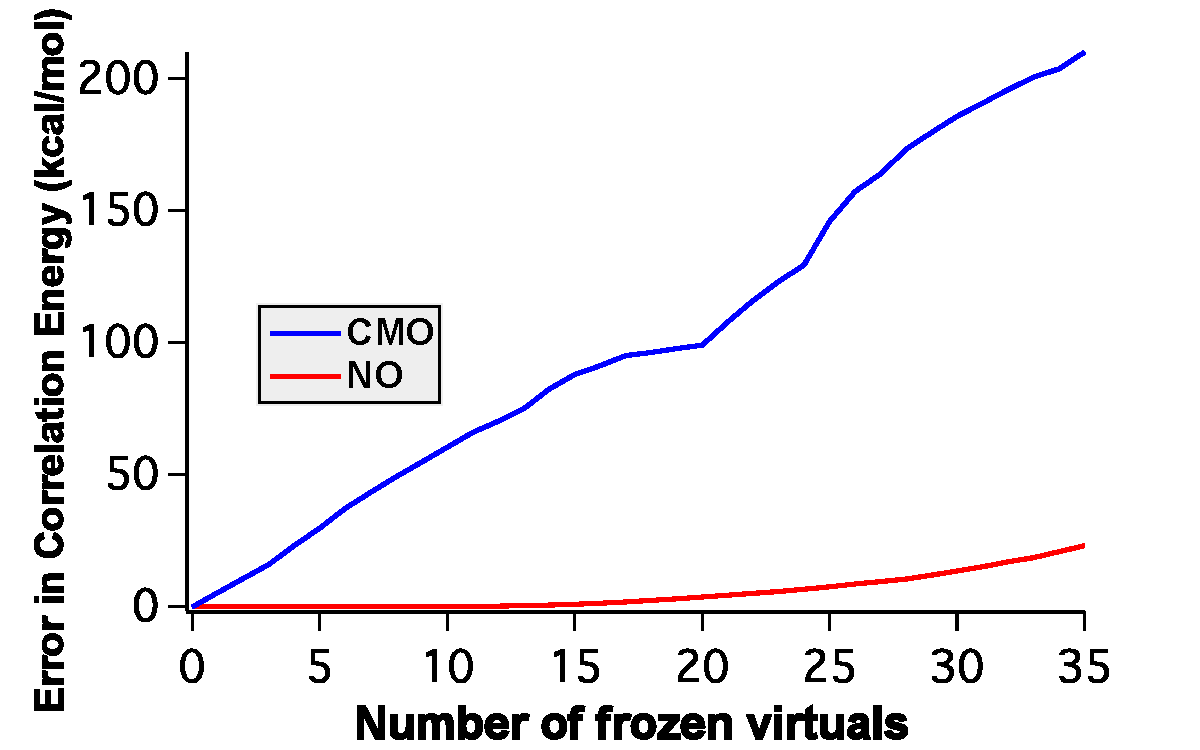
\includegraphics[width=0.6\linewidth]{figures_fvno/energy.eps}
%  \caption{Error in the CCSD energy of H$_2$O$_2$ in kcal/mol as a
%           function of the number of frozen virtual orbitals in both CMO and NO bases.}
%  \label{fig:energy}
%\end{figure}
\begin{MyFigure}[h!]
\centering
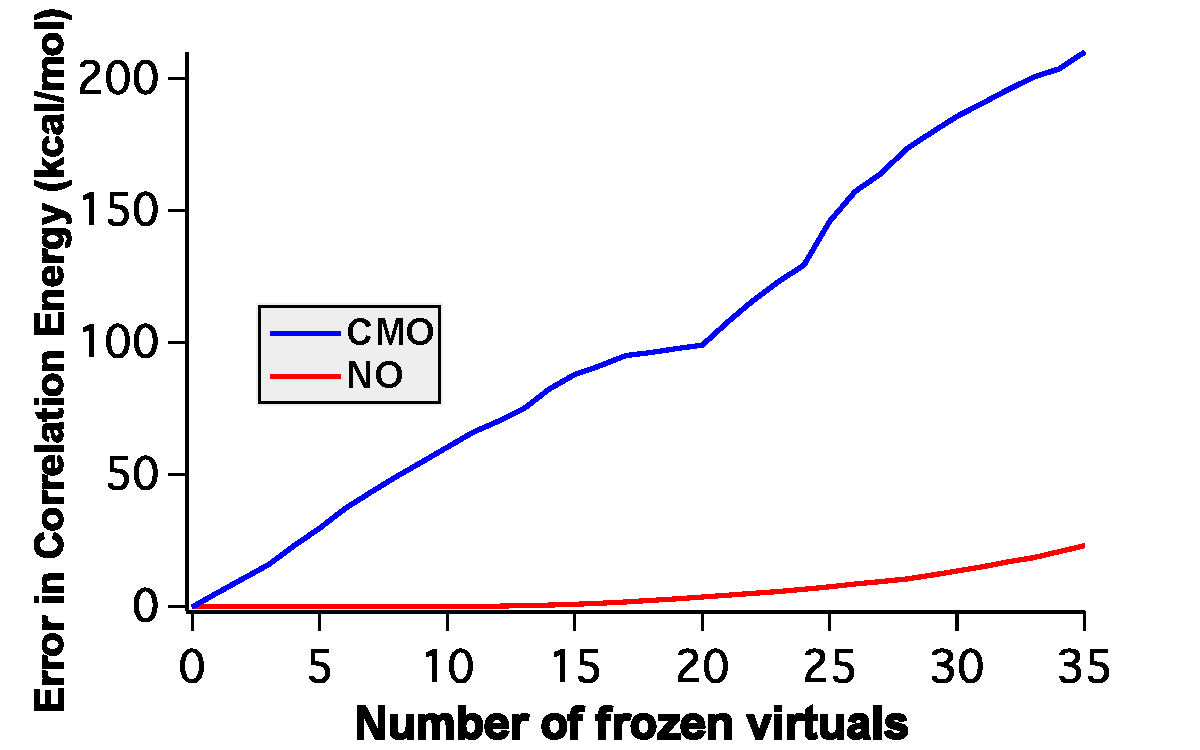
\includegraphics[width=0.6\linewidth]{figures_fvno/energy.pdf}
\caption{{\footnotesize Error in the CCSD energy of H$_2$O$_2$ in kcal/mol as a function of the number of frozen virtual orbitals in both CMO and NO bases.}}
\label{fig:energy}
\end{MyFigure}
plots the error in the CCSD correlation energy of H$_2$O$_2$ in the aDZ basis as a function of
the number of frozen virtual CMOs (removed starting from the highest energy
orbitals) or NOs (starting from the lowest occupation numbers).  Clearly the
correlation energy is very sensitive towards the removal of CMOs, with the
error increasing by more than 4 kcal/mol after the deletion of even one
virtual orbital.  On the other hand, removal of low occupation-number NOs
introduces errors of only ca.\ 2.5 kcal/mol even when up to 33\% of the
virtual space (18 of 55 orbitals) is truncated.  The errors in
the NO basis can be further minimized by employing an MP2 energy correction,
\\
\begin{equation}
E^{\rm MP2}_{\rm corr} = \frac{1}{4} \sum_{ij} \sum_{ab \in {\rm ext}} \frac{|\langle
ij||ab\rangle|^2}{\epsilon_i + \epsilon_j - \epsilon_a - \epsilon_b}.
\label{Eq:MP2}
\end{equation}
\\
where the summation over virtual orbitals is limited to NOs in the external,
truncated space.  Fig.~\ref{fig:MP2_corr} 
\begin{MyFigure}[h!]
\centering
\includegraphics[width=0.6\linewidth,natwidth=610,natheight=642]{figures_fvno/Mp2c.pdf}
\caption{{\footnotesize Error in CCSD energy of H$_2$O$_2$ in the NO bases, with and without MP2 corrections
        and MP2 correction as a function of the number of frozen virtual orbitals.}}
\label{fig:MP2_corr}
\end{MyFigure}
plots the error in the CCSD correlation energy for the same system as above in the NO basis, with and
without this correction (left-hand vertical axis), as well as the correction
itself (right-hand axis).  After employing the correction, the error in the
correlation energy falls to less than 0.1 kcal/mol when 1/3 of the virtual
space is eliminated. Similar results are obtained for aTZ and aQZ basis sets,
where the truncation errors are less than 1 kcal/mol even after the removal of 50\%
of the virtual space. We note that the MP2 energy correction is significant 
(on the order of m$E_h$ or several kcal/mol) even for small compounds such as 
H$_2$O$_2$.  The correction scales linearly with the number of electrons and 
thus is a critical component for the success of the frozen virtual NO approach 
for larger molecules.

\subsection{Frozen Virtual Orbitals and Response Properties}

What is the impact of freezing virtual orbitals --- whether CMO or NO --- on
higher-order properties?  Fig.~\ref{fig:polar_h2o2} 
\begin{MyFigure}[h!]
\centering
\includegraphics[width=0.6\linewidth]{figures_fvno/h2o2_polar.pdf}
\caption{{\footnotesize Errors in the CCSD/aDZ dynamic polarizability (589 nm) of H$_2$O$_2$ in
       in both CMO and NO bases as a function of number of virtual orbitals removed .}}
\label{fig:polar_h2o2}
\end{MyFigure}
plots errors in dynamic polarizabilites (computed at a wavelength of 589 nm) as a function of the
number of virtual orbitals deleted at the CCSD/aDZ level of theory for the
same H$_2$O$_2$ test case as above.  Comparison to Fig.\ \ref{fig:energy}
reveals precisely the opposite behavior for polarizabilities as for
correlation energies, {\em viz.}, truncation of the CMO virtual space induces
much smaller errors than does that of the NO virtual space.  For the latter,
errors increase approximately linearly with the number of frozen virtual NOs.
On the other hand, for the CMO basis, the error increases slowly to a maximum
of 1.9\% when 13 virtual orbitals are removed and then decreases to only
-0.3\% when as many as 27 orbitals (ca.\ 50\% of the virtual space) are
frozen.  This trend is not unique to H$_2$O$_2$ or the aDZ basis set. As shown
in Fig. 6.1 of the Supporting Information, the same behavior is observed for
other molecules such as dimethylallene, methyloxirane, and such compounds
interacting with explicit solvent molecules.  In addition, Figs. 6.2 and 6.3
report the same trends for H$_2$O$_2$ with the larger aTZ and aQZ basis sets.


What is the source of this unexpected behavior?  It is well known that diffuse
basis sets are essential for the accurate descriptions of a variety of
response properties, such as dipole polarizabilities.\cite{Woon94}  Fig.~\ref{fig:spatial}
\begin{MyFigure}[h!]
\centering
\includegraphics[width=0.6\linewidth,natwidth=610,natheight=642]{figures_fvno/spatial.pdf}
\caption{{\footnotesize Spatial extent ($\langle r^2\rangle$) of virtual
orbitals of H$_2$O$_2$ in both CMO and NO bases.  Orbitals are ordered
left-to-right by decreasing energy (CMOs) or increasing occupation number (NOs).}}
\label{fig:spatial}
\end{MyFigure}
plots the spatial extent --- $\langle r^2 \rangle$ --- for each virtual CMO or
NO in the same ordering as they are deleted in Fig.~\ref{fig:polar_h2o2}.  The
Figure clearly shows that the earliest NOs to be removed (the ones with the
lowest occupation numbers) are the most diffuse, {\em i.e.}, they should
contribute substantially to the description of the dynamic polarizability.  On
the other hand, the first CMOs to be frozen (those with the highest orbital
energies) are also the most compact and thus contribute the least to this
property.  Given that highly diffuse basis functions typically contribute
primarily to CMOs with low orbital energies --- often below that of what is
normally considered the true anti-bonding ``LUMO'' --- the latter result is
not surprising; these diffuse CMOs appear to the far right of
Fig.~\ref{fig:spatial} and are thus never deleted, leading to the good
behavior of the CMO truncation in Fig.~\ref{fig:polar_h2o2}.  These same
diffuse basis functions, however, contribute little to the description of
dynamical correlation effects, and thus exhibit very low occupation numbers
upon transformation to the NO virtual space.  Thus, they are truncated first
in the NO basis, yielding the large errors in the polarizability depicted in
Fig.~\ref{fig:polar_h2o2}.

The above observations suggest that, for computing response properties such as
dynamic polarizabilities, an alternative approach to truncation of the virtual
space is to order the orbitals by increasing values of $\langle r^2 \rangle$
rather than by decreasing orbital energies (as is done for CMOs) or increasing
occupation numbers (for NOs).  Fig.~\ref{fig:sort_spatial} 
\begin{MyFigure}[h!]
\centering
\includegraphics[width=0.6\linewidth,natwidth=610,natheight=642]{figures_fvno/sort_spatial.pdf}
\caption{{\footnotesize Spatial extent ($\langle r^2\rangle$) of virtual
orbitals of H$_2$O$_2$ in both CMO and NO bases.  Orbitals are ordered
left-to-right by decreasing energy (CMOs) or increasing occupation number (NOs).}}
\label{fig:sort_spatial}
\end{MyFigure}
plots errors in the CCSD/aDZ dynamic polarizability of H$_2$O$_2$ as the virtual CMOs or NOs are
removed in order of increasing spatial extent.  While the errors are
comparable to that observed in Fig.~\ref{fig:polar_h2o2} for the CMO
truncation, the behavior associated with removal of virtual NOs is
significantly different.  First, the polarizability errors exhibit two
plateaus: one associated with diffuse NOs 2-5 and another with NOs 16-30, and
removal of these NOs has little impact on the observed error.  However,
deletion of the virtual NO with the {\em smallest} spatial extent unexpectedly
leads to a large initial error (ca.\ 7.5 a.u.), followed later by a linearly
increasing error as virtual NOs 6-15 are removed.  Clearly, spatial extent is
not the only criterion by which we may predict the importance of a given
virtual NO to the polarizability.

Another possible source of error is the lack of orbital response in the chosen
formulation of the coupled cluster linear response function.\cite{Koch94:BCC}
In the infinite-lifetime approximation, frequency-dependent properties such as
dipole polarizabilities exhibit first-order poles at the excitation
frequencies.  In the coupled cluster formulation described above, the orbital
response to the external field is typically neglected so that these poles
correspond solely to the response for the correlated wave function, and
additional, spurious poles arising due to the Hartree-Fock reference
determinant will not appear.  (This approximation is typically justified based
on the fact that much of the orbital-response effects are accounted for by the
singles amplitudes\cite{Christiansen95:CC2}.  In order to test whether the
orbital relaxation significantly impacts the behavior of the computed
polarizability as the virtual space is reduced, we have computed {\em static}
($\omega = 0.0$) polarizabilities using finite-differences (with a a
central-difference formula with a differential field strength of 0.001 a.u.)
The errors in the CCSD/aDZ static polarizability of H$_2$O$_2$ for both CMO
and NO virtual spaces are reported in Fig.~\ref{fig:static}.  
\begin{MyFigure}[h!]
\centering
\includegraphics[width=0.6\linewidth,natwidth=610,natheight=642]{figures_fvno/polar_static.pdf}
\caption{{\footnotesize Errors in the CCSD/aDZ static polarizability
(including orbital relaxation effects) of H$_2$O$_2$ in
in both CMO and NO bases as a function of number of virtual orbitals
removed.}}
\label{fig:static}
\end{MyFigure}
Interestingly, with orbital relaxation included, the truncation of the NO space now becomes
better behaved than the CMO space over a large domain of orbitals removed.
Unfortunately, we cannot take advantage of this improvement in conjunction
with Hartree-Fock orbitals without corrupting the pole structure of the
response function.  A Brueckner or orbital-optimized approach may prove
superior in this regard, though further investigation is
warranted.\cite{Koch94:BCC,Pedersen01}

\subsection{Wave Function Truncation in the Virtual-Orbital Space}

For additional insight into the above observations, we examine errors arising
in dynamic polarizabilities as a function of truncation of specific
wavefunction parameters in either the CMO or NO basis.
Fig.~\ref{fig:amp_trunc_cmo} 
\begin{MyFigure}[h!]
\centering
\includegraphics[width=0.6\linewidth,natwidth=610,natheight=642]{figures_fvno/amp_trunc_cmo.pdf}
\caption{{\footnotesize Errors introduced in CCSD/aDZ polarizabilities of
H$_2$O$_2$ in the virtual CMO bases by the truncation of different classes of wave
function amplitudes.}}
\label{fig:amp_trunc_cmo}
\end{MyFigure}
plots the errors in CCSD/aDZ dynamic polarizabilities of H$_2$O$_2$ as a result of truncations of the unperturbed
ground-state cluster amplitudes $\hat{T}$ and $\hat{\Lambda}$, as well as
perturbed amplitudes, $\hat{X}_\omega^\mu$, represented in the CMO basis.
Note that, in this analysis, only the specified amplitudes associated with the
selected CMOs are forced to zero; the CMOs remain active for all other wave
function components.  From the Figure, it can be clearly seen that removing
$\hat{T}_1$ alone does not introduce any significant error in the
polarizability, whereas truncating $\hat{T}_2$ amplitudes results in
substantial positive errors which increase almost linearly with the number of
virtual CMOs. Not surprisingly, freezing both $\hat{T}_1$ and $\hat{T}_2$
amplitudes together have essentially the same effect as freezing $\hat{T}_2$
amplitudes alone. Alternatively, for the left-hand wave function, removing
$\hat{\Lambda}_1$ and $\hat{\Lambda}_2$ amplitudes either separately or
pairwise seems to have negligible impact.  In the case of the perturbed
amplitudes, only small (negative) errors are introduced even after freezing
all $\hat{X}_1$ amplitudes involving almost 23 virtual CMOs, but the error
then rises sharply with further truncation.  On the other hand, the negative
errors due to truncation of $\hat{X}_2$ amplitudes are significant from the
beginning and increase almost linearly.  Thus the error due to removal of both
$\hat{X}_1$ and $\hat{X}_2$ amplitudes belonging to the first 23 CMOs is due
to elimination of $\hat{X}_2$ amplitudes alone, whereas beyond that limit, the
total error corresponds to the sum of errors from $\hat{X}_1$ and $\hat{X}_2$
truncation.

A key observation is that, within the domain of the first 23 virtual CMOs, the
positive errors introduced by truncation of $\hat{T}_2$ are cancelled almost
exactly by the negative errors arising from the truncation of $\hat{X}_2$.
This is further illustrated in Fig.~\ref{fig:error_compare}, 
\begin{MyFigure}[h!]
\centering
\includegraphics[width=0.6\linewidth,natwidth=610,natheight=642]{figures_fvno/error_cmpare.pdf}
\caption{{\footnotesize Errors introduced in CCSD/aDZ polarizabilities of
H$_2$O$_2$ in the virtual CMO bases by the truncation of specific classes of wave
function amplitudes as compared to the total errors obtained by freezing of
virtual CMOs.}}
\label{fig:error_compare}
\end{MyFigure}
which plots on a narrow range the errors in the polarizability associated with truncating
specific classes of $\hat{T}_2$ and $\hat{X}_2$ amplitudes against the total errors
obtained by freezing CMOs entirely (for all amplitudes).  Outside of this
domain, errors associated with neglect of $\hat{X}_1$ amplitudes become
dominant, leading to the accumulation of negative total errors observed in
Fig.~\ref{fig:polar_h2o2}.  Thus, the apparently robust performance of the
truncation of the virtual CMO space arises, in fact, from offsetting
errors.

Similarly to the above analysis for the virtual CMO space,
Fig.~\ref{fig:amp_trunc_no} 
\begin{MyFigure}[h!]
\centering
\includegraphics[width=0.6\linewidth,natwidth=610,natheight=642]{figures_fvno/amp_trunc_no.pdf}
\caption{{\footnotesize Errors introduced in CCSD/aDZ polarizabilities of
H$_2$O$_2$ in the virtual NO bases by the truncation of different classes of wave
function amplitudes.}} 
\label{fig:amp_trunc_no}
\end{MyFigure}
reports errors in the CCSD/aDZ polarizability of
H$_2$O$_2$ introduced by the neglect of various classes of wave function
amplitudes associated with selected virtual NOs.  We observe first that,
unlike the CMO case, neglecting $\hat{T}_2$ amplitudes associated with
particular virtual NOs has no significant effect on the error.  This behavior
is expected, because the $\hat{T}_2$ amplitudes are, by construction, sparse
in the virtual NO basis such that orbitals with low occupation numbers are
associated with $\hat{T}_2$ amplitudes of smaller magnitude.  Furthermore,
just as in the CMO case, the removal of $\hat{T}_1$, $\hat{\Lambda}_1$ and
$\hat{\Lambda}_2$ amplitudes introduces only small errors, while the removal
of selected $\hat{X}_2$ amplitudes based on NOs yields significant negative
errors that increase linearly with the number of virtual NOs truncated.

However, unlike the virtual CMO case, neglecting $\hat{X}_1$ amplitudes
corresponding to specific virtual NOs introduces large negative errors in the
polarizability even from the first NO removed, and the total error obtained by
truncating both $\hat{X}_1$ and $\hat{X}_2$ amplitudes is almost the same as
the error due to truncation of the $\hat{X}_1$ amplitudes alone.  Indeed, 
the greatest contribution ($>90\%$) to the
total polarizability errors arises from the perturbed singles amplitudes.

The significance of the $\hat{X}_1$ amplitudes is evident upon analysis of
their leading-order contribution to the polarizability [cf.\
Eq.~(\ref{Eq:alpha})],
\\
\begin{equation}
\alpha_\omega \leftarrow \frac{1}{3} \sum\limits_{ia}\sum\limits_x \mu^{x}_{ia}(X^x_{ia}(\omega) +
X^x_{ia}(-\omega)),
\label{Eq:leading_X1}
\end{equation} 
\\
where $\mu^x_{ia}$ is an element of the occupied-virtual block of the
Cartesian component, $x$, of the electric-dipole moment integral matrix, and the inner
sum runs over all such components. The singles
themselves are obtained from the corresponding form of
Eq.~(\ref{Eq:perturbed_wfn}),
\\
\begin{equation} 
\langle\Psi^a_i|X^{\mu}_{\omega}|\Psi_0\rangle =
-\sum_{\nu}\langle\Psi^a_i|(\bar{H} -
\omega)^{-1}|\nu\rangle\langle\nu|\bar{\mu}|\Psi_0\rangle,
\hspace{0.15in}\nu
\in \{\Psi^b_j,\Psi^{cd}_{jk}\},
\label{Eq:singles}
\end{equation} 
\\
where $\bar{\mu}$ is the similarity transformed electric-dipole operator,
\\
\begin{equation}
\bar{\mu} = \hat{\mu} + \bigg[\hat{\mu},\hat{T}\bigg] +
\frac{1}{2}\bigg[\bigg[\hat{\mu},\hat{T}\bigg],\hat{T}\bigg].
\label{Eq:mubar}
\end{equation}
\\
The corresponding leading-order contribution to the $\hat{X}_1$ amplitudes themselves is
\\
\begin{equation}
X^{\mu}_{ia}(\omega) \leftarrow \frac{\mu_{ia}}{\overbar{H}_{ii} -
\overbar{H}_{aa} + \omega},
\label{Eq:X1}
\end{equation}
\\
where the largest contribution to the diagonal elements of the similarity
transformed Hamiltonian, $\bar{H}$, arises from the orbital energies (more
precisely, the diagonal Fock matrix elements expressed in the CMO or NO
basis), which are plotted in Fig.~\ref{fig:Faa}. 
\begin{MyFigure}[h!]
\centering
\includegraphics[width=0.6\linewidth,natwidth=610,natheight=642]{figures_fvno/Faa.pdf}
\caption{{\footnotesize Virtual diagonal elements (a.u.) of the Fock matrix (F) in
the CMO and NO bases.}}
\label{fig:Faa}
\end{MyFigure}
While the values for the virtual CMOs decrease steadily, their NO counterparts actually {\em increase}
and display greater oscillation.  Clearly, the diagonal elements of the Fock
matrix for virtual NOs are significantly smaller in magnitude than the
corresponding CMOs, which concomitantly increases the values of the
$\hat{X}_1$ amplitudes associated with such NOs.  This effect can be seen in
Fig.~\ref{fig:X1} 
\begin{MyFigure}[h!]
\centering
\includegraphics[width=0.6\linewidth,natwidth=610,natheight=642]{figures_fvno/X1.pdf}
\caption{{\footnotesize  Sum of the absolute values of $\hat{X}_1$
amplitudes for a given virtual, $\sum_i \left|X_i^a\right|$, for perturbation $\mu_x$
and frequency 589 nm, plotted for each virtual NO or CMO.}}
\label{fig:X1}
\end{MyFigure}
which plots the sum of the absolute values of $\hat{X_1}$
amplitudes for a given virtual orbital, i.e.  $\sum_i |X_i^a|$, for both
virtual CMOs and NOs.  Thus, the sparsity of the $\hat{X}_1$ amplitudes present in the
CMO basis is almost completely lost in the NO basis, which leads to the large
errors in dynamic polarizabilities due to the truncation of $\hat{X}_1$
amplitudes in the NO basis observed earlier.  

Furthermore, the dependence of the $\hat{X}_1$ amplitudes on both $\hat{T}_2$
and $\hat{X}_2$ plays a significant role in the overall {\em sign} of the
polarizability error.  This point is clearly illustrated in
Fig.~\ref{fig:norm}, 
\begin{MyFigure}[h!]
\centering
\includegraphics[width=0.6\linewidth,natwidth=610,natheight=642]{figures_fvno/norm.pdf}
\caption{{\footnotesize The 2-norm of the $\hat{X}_1$ amplitude vector in
the CMO bases as a function of the truncation of classes of unperturbed
$\hat{T}_2$ and perturbed $\hat{X}_2$ amplitudes. }}
\label{fig:norm}
\end{MyFigure}
which plots the 2-norm of the $\hat{X}_1$ vector as
$\hat{T}_2$ or $\hat{X}_2$ amplitudes associated with a given virtual CMO are
neglected (in the same manner as used in Figs.~\ref{fig:amp_trunc_cmo} and
\ref{fig:error_compare}). As the $\hat{T}_2$ amplitudes associated with a given
virtual orbital are removed, the norm of the $\hat{X}_1$ vector
increases, leading to the positive errors in the polarizability observed in
Fig.~\ref{fig:amp_trunc_cmo}.  On the other hand, removal of $\hat{X}_2$
amplitudes leads to a decrease in the norm of the $\hat{X}_1$ vector and
the negative errors in the polarizability appearing in
Fig.~\ref{fig:amp_trunc_cmo}.

\subsection{External-Space Corrections}

As noted earlier, a key aspect of the strong performance of virtual NOs for
correlation energies is the use of MP2-based corrections for the contributions
of the truncated or ``external'' virtual space, as given in
Eq.~(\ref{Eq:MP2}).  When considering a similar correction for properties,
however, we have explored three options: time-dependent Hartree-Fock (TDHF)
and both static and dynamic CC2\cite{Christiansen95:CC2} corrections.  In each
case, we have used the same MP2-based virtual NO space and computed the
correction as the difference between the full-virtual space polarizability and
the truncated virtual-NO polarizability, with the CCSD/aDZ results for
polarizabilties of H$_2$O$_2$ shown in Fig.~\ref{fig:corrections}.
\begin{MyFigure}[h!]
\centering
\includegraphics[width=0.6\linewidth,natwidth=610,natheight=642]{figures_fvno/correctn.pdf}
\caption{{\footnotesize Correction schemes for the external truncated
NO space for the CCSD/aDZ polarizabilities of H$_2$O$_2$.}}
\label{fig:corrections}
\end{MyFigure}
The CC2-based corrections recover nearly all of the error associated with the
uncorrected virtual NO space across a wide range of truncation, with the
static correction actually yielding slightly smaller errors than its dynamic
counterpart.  The less expensive TDHF corrections offer significant
improvement over the original virtual NO results, and recover most (ca.\ 85\%)
of the error until about 40\% (21 orbitals) of the virtual space has been
deleted, but they clearly produce overall larger errors than the correlated
methods.  In addition, the TDHF corrections are potentially problematic
because the pole structure of the polarizability naturally follows that of the
underlying Hartree-Fock perturbed orbitals rather than that of the correlated
wave functions,\cite{Aiga96,Hattig95,Rice91} a criticism that would also hold
for purely MP2-based corrections.  On the other hand, the CC2-based
corrections are significantly more expensive than TDHF, in part because of
their iterative nature and the
need to transform two-electron integrals involving three virtual orbitals
(with the latter criticism again holding for an MP2-based correction).

\subsection{Perturbed Natural Orbitals}

Given that the purpose of the NOs is to ``focus'' the important components of
the basis for the description of electron correlation effects into a compact
space, without consideration of the importance of the basis set for other
properties, an alternative approach might be to build a virtual space that
explicitly takes such properties into account, such as the inclusion of the
perturbed one-electron density in the definition of the space.  Instead of
diagonalizing the ground-state MP2 density, we diagonalize its gradient with
respect to the external electric field, thereby incorporating the effects of
the external perturbations.  The resulting ``occupation numbers'' obtained
thus carry information about orbital occupancies in the perturbed states.  The
$x^{th}$ Cartesian component of the perturbed density matrix can be written in
terms of spin orbitals as
\\
\begin{equation}
\gamma^x_{ab} = \frac{1}{2}\sum_{ijc}P_{+}(a,b)\left[\frac{t^{bc}_{ij}}{D^{ac}_{ij}} \
\left(P_{-}(a,c)\sum_dt^{ad}_{ij}\mu^x_{cd} - P_{-}(i,j)\sum_m t^{ac}_{im}\mu^x_{mj}\right)\right]
\label{Eq:perturb_d}
\end{equation}
\\
where $P_{+}$ and $P_{-}$ are symmetric and anti-symmetric permutation
operators, respectively, and the orbital-energy denominator $D^{ac}_{ij} =
\epsilon_i + \epsilon_j  -\epsilon_a -\epsilon_c $.  (For computational
convenience, orbital relaxation terms have been neglected.) To obtain the
perturbed NOs and their corresponding eigenvalues, we take an average of the
three cartesian components of the density and diagonalize the result.
The eigenvalues consist of both positive and negative values as the perturbed
density matrix is not positive definite, and thus we truncate the orbitals
based on the absolute values of these eigenvalues.
Fig.~\ref{fig:perturb} 
\begin{MyFigure}[h!]
\centering
\includegraphics[width=0.6\linewidth,natwidth=610,natheight=642]{figures_fvno/perturbed.pdf}
\caption{{\footnotesize Errors introduced in CCSD/aDZ polarizabilities of
H$_2$O$_2$ in the virtual CMO and NO bases, as well as the perturbed
virtual NO basis as a function of number of virtual orbitals removed.}}
\label{fig:perturb}
\end{MyFigure}
compares the performance of these perturbed NOs with
that of the CMOs and NOs, where the error in the CCSD/aDZ dynamic
polarizability of H$_2$O$_2$ is plotted as a function of the number of virtual
orbitals removed. While the perturbed NOs lower the truncation errors
associated with conventional NOs, they still introduce significantly higher
errors than the corresponding CMOs.  The reason for this underperformance is
related to the definition of the perturbed density, which naturally bears
strong similarity to its unperturbed counterpart [cf. Eqs.~(\ref{Eq:dens}) and
(\ref{Eq:perturb_d})]. As a result, similar sparsity and orbital energy issues
illustrated in Figs.~\ref{fig:Faa} and \ref{fig:X1} arise for the perturbed
density just as for the original NOs, indicating that such an approach does not
resolve the problem.

\subsection{The Dipole-Amplitude Criterion}

The above results demonstrate that the CMO basis provides the best performance
among the various virtual spaces considered here, albeit based on cancellation
of errors. But what criterion should be used to determine the truncation level
that provides optimal balance between computational cost (most compact virtual
space) and accuracy?  The CMO orbital energies are one possibility, but they
have no direct connection to the properties in question.  Another alternative
is the ``dipole amplitude'', $d_a$, which is defined for each virtual CMO as
\\
\begin{equation}
d_a \equiv \sum\limits_x\sum\limits_i\frac{({\mu^x_{ia}})^2}{\epsilon_i - \epsilon_a}.
\label{Eq:dipole}
\end{equation}
\\
This expression, which is trivially computed post-Hartree-Fock, is based on
Eqs.~(\ref{Eq:leading_X1}) and (\ref{Eq:X1}), using the fact that the leading
contributions to the diagonal elements of the similarity-transformed
Hamiltonian are the orbital energies.    As we are constructing a
phenomenological truncation criterion, we have chosen to neglect the
dependence on the field frequency.
Fig.~\ref{fig:dipole_length} 
\begin{MyFigure}[h!]
\centering
\includegraphics[width=0.6\linewidth,natwidth=610,natheight=642]{figures_fvno/diplength.pdf}
\caption{{\footnotesize Absolute errors introduced in CCSD/aDZ
  polarizabilities of H$_2$O$_2$ due to truncation of $\hat{X}_1$ amplitudes and
  dipole amplitudes plotted as a function of different virtual CMOs.}}
\label{fig:dipole_length}
\end{MyFigure}
plots the values of the dipole amplitude for
each CMO, as well as the corresponding error in the CCSD/aDZ
dipole-polarizability of H$_2$O$_2$ introduced by deleting the $\hat{X}_1$
amplitude associated with a given virtual CMO. There is a clear correlation
between the two functions, and one can see that as both the error due to
truncation of $\hat{X}_1$ and the value of the dipole amplitude increase sharply
once we reach CMOs 27-28 --- ca. 50\% of the virtual space for this test case.
Accordingly, one should stop the truncation of the virtual CMO space once the
dipole amplitude values start rising sharply.  While the optimal choice of
such a threshold will be addressed systematically in subsequent work, our
preliminary analyses using H$_2$O$_2$, methyloxirane, dimethylallene, and
related compounds suggest a cutoff of ca.\ 3-3.5\% (of the total dipole amplitude) 
yields minimal errors in the polarizability.

\section{Conclusions}

On the basis of the above findings, we conclude that, in the absence of
orbital relaxation, virtual NOs are not
suited for higher-order property calculations such as dynamic
polarizabilities, and that the occupation number is not an acceptable
criterion for estimating the importance of a virtual orbital for such
calculations.  Although the use of external space corrections based on CC2
polarizabilities reduces the observed truncation errors, they are too
relatively costly to be practical for large molecular systems.  Furthermore,
the use of perturbed virtual NOs offers only slight improvement as compared to
unperturbed virtual NOs.  CMOs, on the other hand, provide a much more stable
mechanism for reducing the size of the virtual space --- with truncation of up
to 50\% of the orbitals yielding shifts of less than 2\% as compared to
full-space calculation -- but the source of their success lies in a
significant cancellation of errors.  Although further systematic studies are
needed, the dipole amplitude appears to provide a useful threshold for an {\em
a priori} truncation of the CMO virtual space.

%\section{Acknowledgements}
%
%This research was supported by a grant (CHE-1465149) from the U.S.\
%National Science Foundation. The authors acknowledge Advanced Research
%Computing at Virginia Tech for providing computational resources and
%technical support that have contributed to the results reported within this
%paper.

\clearpage
%\bibliographystyle{rsc}
%\bibliography{refs}

\newpage

%%%%%%%%%%%%%%%%%%%%%%%%%%%%%%%%%%%%%%%%%%%%%%%%%%%%%%%%%%%%%%%%%
\begin{figure}
  \centering
  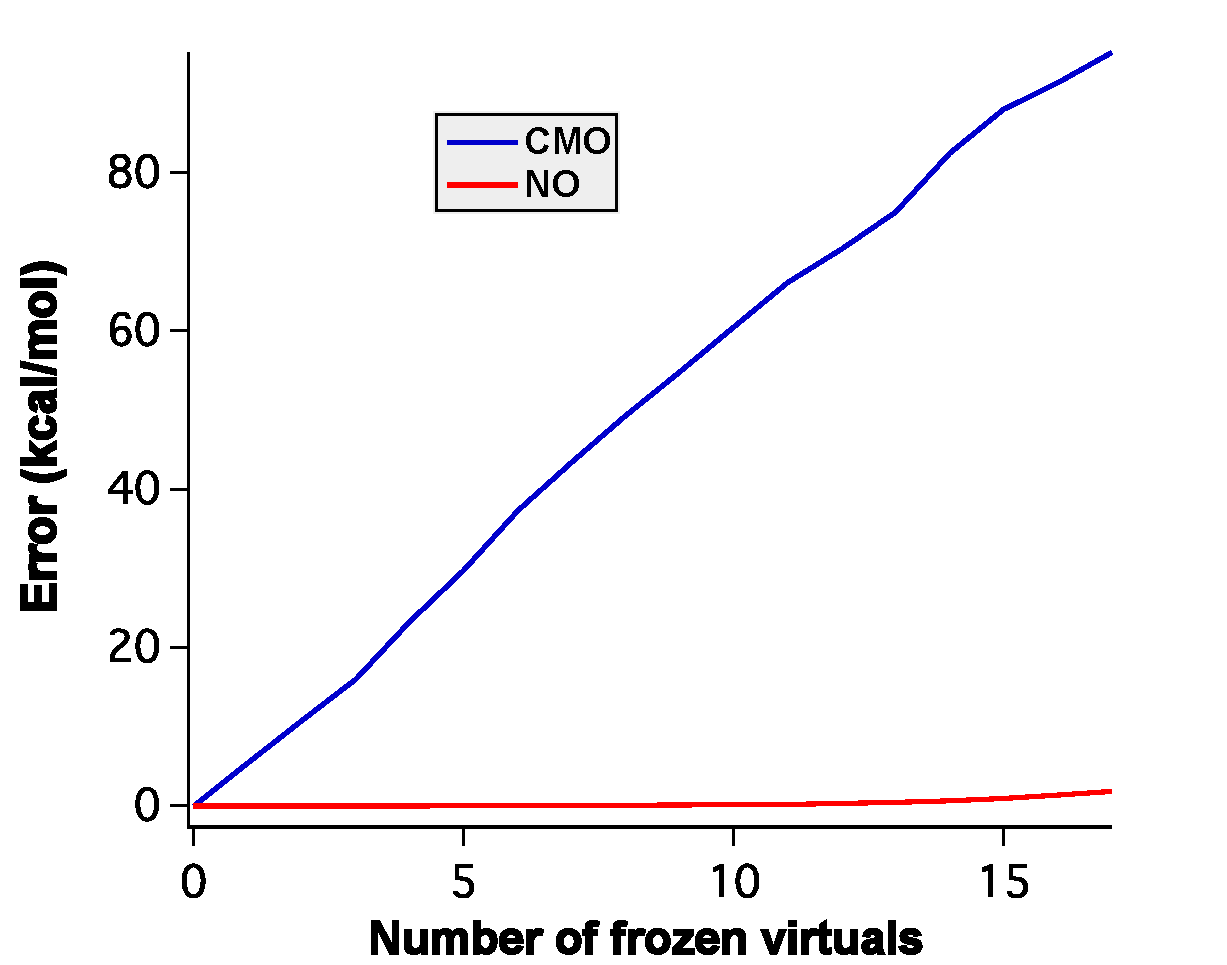
\includegraphics[width=0.7\linewidth]{figures/energy.pdf}
  \caption{Error in the CCSD energy of H$_2$O$_2$ in kcal/mol as a 
           function of the number of frozen virtual orbitals in both CMO and NO bases.} 
  \label{fig:energy}
\end{figure}
%%%%%%%%%%%%%%%%%%%%%%%%%%%%%%%%%%%%%%%%%%%%%%%%%%%%%%%%%%%%%%%
\begin{figure}
  \centering
  \includegraphics[width=0.7\linewidth]{figures/Mp2c.pdf}
  \caption{Error in CCSD energy of H$_2$O$_2$ in the NO bases, with and without MP2 corrections 
        and MP2 correction as a function of the number of frozen virtual orbitals.}
\label{fig:MP2_corr}
\end{figure}
%%%%%%%%%%%%%%%%%%%%%%%%%%%%%%%%%%%%%%%%%%%%%%%%%%%%%%%%%%%%%%%
\begin{figure}
  \centering
  \includegraphics[width=0.6\linewidth]{figures/h2o2_polar.pdf}
  \caption{Errors in the CCSD/aDZ dynamic polarizability (589
nm) of H$_2$O$_2$ in 
       in both CMO and NO bases as a function of number of virtual orbitals removed.}
   \label{fig:polar_h2o2}
\end{figure}
%%%%%%%%%%%%%%%%%%%%%%%%%%%%%%%%%%%%%%%%%%%%%%%%%%%%%%%%%%%%%%%
\begin{figure}
  \centering
  \includegraphics[width=0.6\linewidth]{figures/spatial.pdf}
  \caption{Spatial extent ($\langle r^2\rangle$) of virtual
orbitals of H$_2$O$_2$ in both CMO and NO bases.  Orbitals are ordered
left-to-right by
decreasing energy (CMOs) or increasing occupation number (NOs).}
   \label{fig:spatial}
\end{figure}

%%%%%%%%%%%%%%%%%%%%%%%%%%%%%%%%%%%%%%%%%%%%%%%%%%%%%%%%%%%%%%%
\begin{figure}
  \centering
  \includegraphics[width=0.6\linewidth]{figures/polar_static.pdf}
  \caption{Errors in the CCSD/aDZ static polarizability 
(including orbital relaxation effects) of H$_2$O$_2$ in
       in both CMO and NO bases as a function of number of virtual orbitals
removed.}
   \label{fig:static}
\end{figure}

%%%%%%%%%%%%%%%%%%%%%%%%%%%%%%%%%%%%%%%%%%%%%%%%%%%%%%%%%%%%%%%
\begin{figure}
  \centering
  \includegraphics[width=0.6\linewidth]{figures/sort_spatial.pdf}
  \caption{Errors in the CCSD/aDZ dynamic polarizability (589
nm) of H$_2$O$_2$ as a function of the number of virtual CMOs or NOs deleted,
ordered by increasing spatial extent, $\langle r^2 \rangle$.}
   \label{fig:sort_spatial}
\end{figure}
%%%%%%%%%%%%%%%%%%%%%%%%%%%%%%%%%%%%%%%%%%%%%%%%%%%%%%%%%%%%%%%
\begin{figure}
  \centering
  \includegraphics[width=0.6\linewidth]{figures/amp_trunc_cmo.pdf}
  \caption{Errors introduced in CCSD/aDZ polarizabilities of
H$_2$O$_2$ in the virtual CMO bases by the truncation of different classes of wave
function amplitudes.}
   \label{fig:amp_trunc_cmo}
\end{figure}
%%%%%%%%%%%%%%%%%%%%%%%%%%%%%%%%%%%%%%%%%%%%%%%%%%%%%%%%%%%%%%%
\begin{figure}
  \centering
  \includegraphics[width=0.6\linewidth]{figures/error_cmpare.pdf}
  \caption{Errors introduced in CCSD/aDZ polarizabilities of
H$_2$O$_2$ in the virtual CMO bases by the truncation of specific classes of wave
function amplitudes as compared to the total errors obtained by freezing of
virtual CMOs.}
   \label{fig:error_compare}
\end{figure}
%%%%%%%%%%%%%%%%%%%%%%%%%%%%%%%%%%%%%%%%%%%%%%%%%%%%%%%%%%%%%%%
\begin{figure}
  \centering
  \includegraphics[width=0.6\linewidth]{figures/amp_trunc_no.pdf}
  \caption{Errors introduced in CCSD/aDZ polarizabilities of
H$_2$O$_2$ in the virtual NO bases by the truncation of different classes of wave
function amplitudes.}
   \label{fig:amp_trunc_no}
\end{figure}
%%%%%%%%%%%%%%%%%%%%%%%%%%%%%%%%%%%%%%%%%%%%%%%%%%%%%%%%%%%%%%%
\begin{figure}
  \centering
  \includegraphics[width=0.6\linewidth]{figures/Faa.pdf}
  \caption{Virtual diagonal elements (a.u.) of the Fock matrix in
the CMO and NO bases.}
   \label{fig:Faa}
\end{figure}
%%%%%%%%%%%%%%%%%%%%%%%%%%%%%%%%%%%%%%%%%%%%%%%%%%%%%%%%%%%%%%%
\begin{figure}
  \centering
  \includegraphics[width=0.6\linewidth]{figures/X1.pdf}
  \caption{Sum of the absolute values of $\hat{X}_1$
amplitudes for a given virtual, $\sum_i \left|X_i^a\right|$, for perturbation $\mu_x$
and frequency 589 nm, plotted for each virtual NO or CMO.}
   \label{fig:X1}
\end{figure}
%%%%%%%%%%%%%%%%%%%%%%%%%%%%%%%%%%%%%%%%%%%%%%%%%%%%%%%%%%%%%%%
\begin{figure}
  \centering
  \includegraphics[width=0.6\linewidth]{figures/norm.pdf}
  \caption{The 2-norm of the $\hat{X}_1$ amplitude vector in
the CMO bases as a function of the truncation of classes of unperturbed 
$\hat{T}_2$ and perturbed $\hat{X}_2$ amplitudes.}
   \label{fig:norm}
\end{figure}
%%%%%%%%%%%%%%%%%%%%%%%%%%%%%%%%%%%%%%%%%%%%%%%%%%%%%%%%%%%%%%%
%\begin{figure}
%  \centering
%  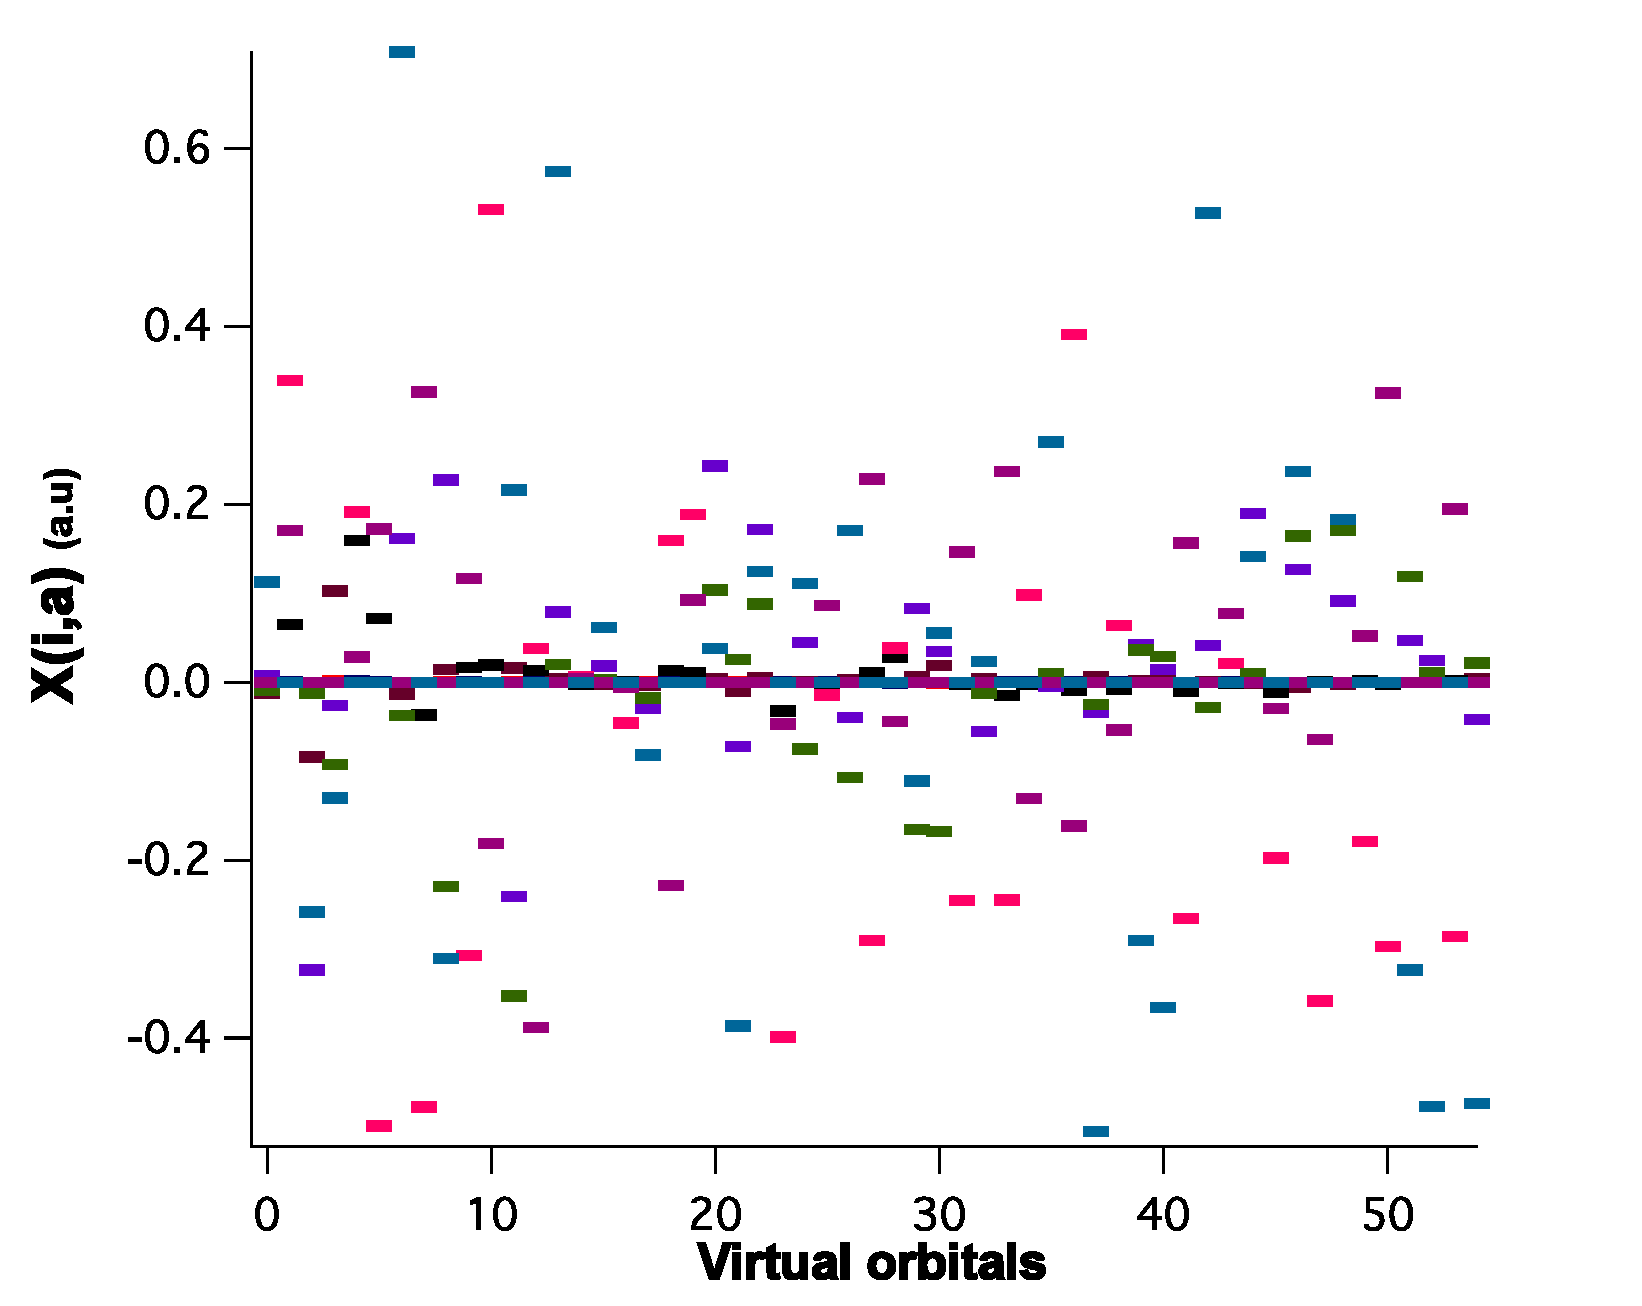
\includegraphics[width=0.6\linewidth]{figures/X1_no.pdf}
%  \caption{\footnotesize{$X_1$ amplitudes $X^{\mu_x}_{ia}$(589 nm) in the NO basis. For each virtual orbital there are nine virtual-occupied pairs.}}
%   \label{fig:X1_no}
%\end{figure}
%%%%%%%%%%%%%%%%%%%%%%%%%%%%%%%%%%%%%%%%%%%%%%%%%%%%%%%%%%%%%%%
\begin{figure}
  \centering
  \includegraphics[width=0.6\linewidth]{figures/correctn.pdf}
  \caption{Correction schemes for the external truncated
NO space for the CCSD/aDZ polarizabilities of H$_2$O$_2$.}
   \label{fig:corrections}
\end{figure}
%%%%%%%%%%%%%%%%%%%%%%%%%%%%%%%%%%%%%%%%%%%%%%%%%%%%%%%%%%%%%%%

\begin{figure}
  \centering
  \includegraphics[width=0.6\linewidth]{figures/perturbed.pdf}
  \caption{Errors introduced in CCSD/aDZ polarizabilities of
H$_2$O$_2$ in the virtual CMO and NO bases, as well as the perturbed
virtual NO basis as a function of number of virtual orbitals removed.}
   \label{fig:perturb}
\end{figure}
%%%%%%%%%%%%%%%%%%%%%%%%%%%%%%%%%%%%%%%%%%%%%%%%%%%%%%%%%%%%%%%
\begin{figure}
  \centering
  \includegraphics[width=0.6\linewidth]{figures/diplength.pdf}
  \caption{Absolute errors introduced in CCSD/aDZ
  polarizabilities of H$_2$O$_2$ due to truncation of $\hat{X}_1$ amplitudes and
  dipole amplitudes plotted as a function of different virtual CMOs.}
   \label{fig:dipole_length}
\end{figure}
%%%%%%%%%%%%%%%%%%%%%%%%%%%%%%%%%%%%%%%%%%%%%%%%%%%%%%%%%%%%%%%


\newpage
\begin{center}
{\bf TOC Graphic}
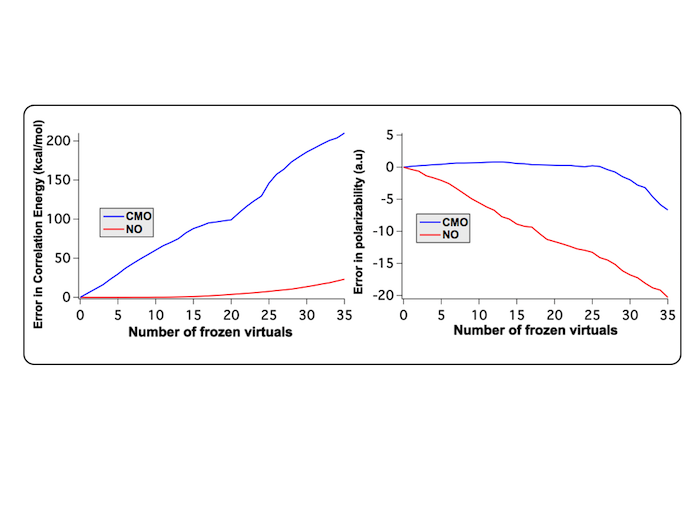
\includegraphics[width=1.0\linewidth]{figures/toc.png}
\end{center}


%\end{document}
